\documentclass[10pt]{beamer}

\usetheme{metropolis}
\usepackage{appendixnumberbeamer}

\usepackage{booktabs}
\usepackage[scale=2]{ccicons}

\usepackage{pgfplots}
\usepgfplotslibrary{dateplot}

\usepackage{xspace}
\newcommand{\themename}{\textbf{\textsc{metropolis}}\xspace}

\title{Detecting Malicious Shell Commands}
\subtitle{A review of text classification techniques}
\date{\today}
\author{rdube}
% \institute{Center for modern beamer themes}
% \titlegraphic{\hfill\includegraphics[height=1.5cm]{logo.pdf}}


\begin{document}

\maketitle

\begin{frame}{Table of contents}
  \setbeamertemplate{section in toc}[sections numbered]
  \tableofcontents[hideallsubsections]
\end{frame}

\section{Motivation}

\begin{frame}[fragile]{Why study this topic?}
	Several reasons to study the topic:
	\begin{itemize}
		\item PowerShell increasingly used in attacks \cite{symc2016}
		\item (In general) Fileless attack techniques increasing \cite{symc2017}
		\item Scripts becoming weapons of choice for sophisticated attack groups \cite{msft2017-2}
		\begin{itemize}
			\item Fileless techniques used during the SolarWinds hack \cite{volexity2020,zdnet2021}
		\end{itemize}
		\item Complicated and obfuscated scripts difficult for human analysts to decipher \cite{feye2018}
	\end{itemize}
\end{frame}

\begin{frame}{What is fileless malware?}
	Fileless malware definition (adapted from \cite{symc2017}):
	\begin{itemize}
		\item Only pre-installed software is used, and no additional binary executables are installed onto the system by the attacker (no files are written to disk)
		\item E.g., VBscript, PowerShell scripts, or the use of system commands, such as netsh commands
		\item E.g., Memory only shellcode dropped by an exploit, which does not write any files on disk
		\item E.g., Brute-forcing the password for Remote Desktop Protocol (RDP) access
	\end{itemize}
\end{frame}

\begin{frame}{Malicious shell commands are a subset of fileless malware}
	Malicous command-line is:
	\begin{itemize}
		\item Defined solely in terms of analyses of objects and (external) verdicts on the analyses
		\item A command-line is malicious if it only appears in analyses deemed malicious
		\item A command-line is benign if it only appears in analyses deemed benign
		\item A command-line that appears in both malicious and benign analyses is declared malicious if ... \textcolor{red}{needs to be defined}
	\end{itemize}
\end{frame}

\section{Binary command-line model design considerations}

\begin{frame}[fragile]{Major decision points}
	\begin{itemize}
		\item Input data source
		\item Classifier design
	\end{itemize}

	The model design space (under the above headings) is large \cite{survey2021,msft2017,powershell2018,amsi2019,feye2018,feye2018-2,charcnn2016,charcnn2019,transformers2019}:
\end{frame}

\begin{frame}{Input data source considerations (1) ...}
	(In general) the most appropriate techniques will vary depending on input \cite{msft2017-2,msft2019,feye2018}:
	\begin{itemize}
		\item PowerShell vs. VBScript vs. Javascript code 
		\item Single command (could be multiple lines) vs. multiple processes
		\item Raw script vs. that obtained through AMSI or sandbox (if different from raw)
		\item Obfuscated vs. de-obfuscated script
		\item Additional corpora of scripts
		\begin{itemize}
			\item Unlabeled PowerShell scripts from PowerShell Gallery \cite{data1}
			\item Labeled (wrt obfuscation) and unlabeled PowerShell scripts: 408K total including 7K manually labeled \cite{data21,data22}
			\begin {itemize}
				\item Overlaps with PowerShell Gallery
			\end {itemize}
		\end{itemize}
	\end{itemize}
\end{frame}

\begin{frame}{Input data source considerations (2) ...}
	Prior work raises several questions regarding pre-processing data \cite{powershell2018,amsi2019,feye2018}:
	\begin{itemize}
		\item Mechanism to declare a label malicious?
		\item De-obfuscate script coded in base64 (and other) encodings?
		\item Normalize scripts using different IP addresses?
		\item Normalize scripts using random file names?
		\item Normalize abbreviations?
		\item What demarcation to use between tokens?
		\item Eliminate rare tokens?
		\item De-duplicate scripts via clustering and representative selection?
	\end{itemize}
	But, pre-processing depends partially on the type of model chosen
\end{frame}

\begin{frame}{Classifier design considerations...}
	\begin{itemize}
		\item Token-based features vs. character-based features
		\begin{itemize}
			\item For token-based features
			\begin{itemize}
				\item Encoding (bag-of-words) vs. embedding
				\item Inline embedding vs. externally learned embedding
				\item Word2Vec vs. FastText vs. something else
			\end{itemize}
			\item For character-based features
			\begin{itemize}
				\item Encode each character (bag-of-characters) vs something else
			\end{itemize}
		\end{itemize}
		\item Manual-feature extraction vs. automatic feature extraction
		\begin{itemize}
			\item For automatic feature extraction
			\begin{itemize}
				\item CNN vs. self-attention (to extract features from a segment of the command-line)
				\item LSTM vs. position-embedding (to combine signals from sequences of features)
			\end{itemize}
		\end{itemize}
		\item Ensembling technique
		\begin{itemize}
			\item Combine output of individual classifiers vs. combine classifiers inline (i.e., train classifiers together)
		\end{itemize}
	\end{itemize}
\end{frame}

\section{Understanding prior work on malicious command-line detection}

\begin{frame}[fragile]{Extract coherent lego blocks}
	\begin{itemize}
		\item charCNN classifier \cite{charcnn2016,charcnn2019,powershell2018}
		\item CNN-LSTM classifier \cite{amsi2019}
		\item charCNN + CNN-LSTM classifier \cite{amsi2019}
		\item Character-level 3-gram + TF-IDF + Logistic regression \cite{amsi2019}
		\item Obfuscation detector \cite{feye2018}
	\end{itemize}
\end{frame}

\begin{frame}{Lego block 1: charCNN (1)}
	\begin{figure}
		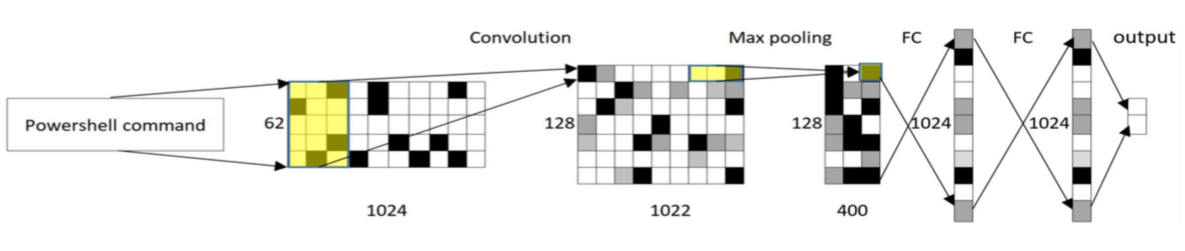
\includegraphics[scale=0.28]{charcnn}
		\caption{Text CNN model as used in \cite{powershell2018}}
	\end{figure}
\end{frame}

\begin{frame}{Lego block 1: charCNN (2)}
	Classifier design:
	\begin{itemize}
		\item Character encoding (bag-of-characters)
		\item CNN to extract features
		\item No explicit mechanism to learn from sequences
	\end{itemize}
\end{frame}

\begin{frame}{Lego block 2: CNN-LSTM (1)}
	\begin{figure}
		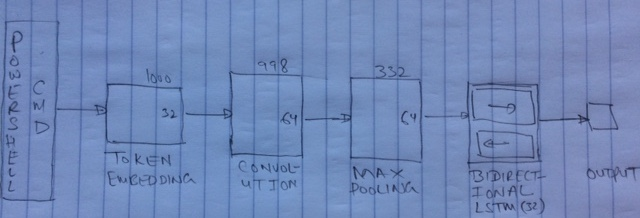
\includegraphics[scale=0.50]{cnn-lstm}
		\caption{CNN-LSTM model as used in \cite{amsi2019}}
	\end{figure}
\end{frame}

\begin{frame}{Lego block 2: CNN-LSTM (2)}
	Classifier design:
	\begin{itemize}
		\item Token based
		\begin{itemize}
			\item FastText embedding from tokens
			\item Externally learned embedding
		\end{itemize}
		\item CNN to extract features
		\item LSTM to learn from sequences of features
		\begin{itemize}
			\item Difficult to parallelize training
		\end{itemize}
	\end{itemize}
\end{frame}

\begin{frame}{Lego block 3: charCNN + CNN-LSTM (1)}
	\begin{figure}
		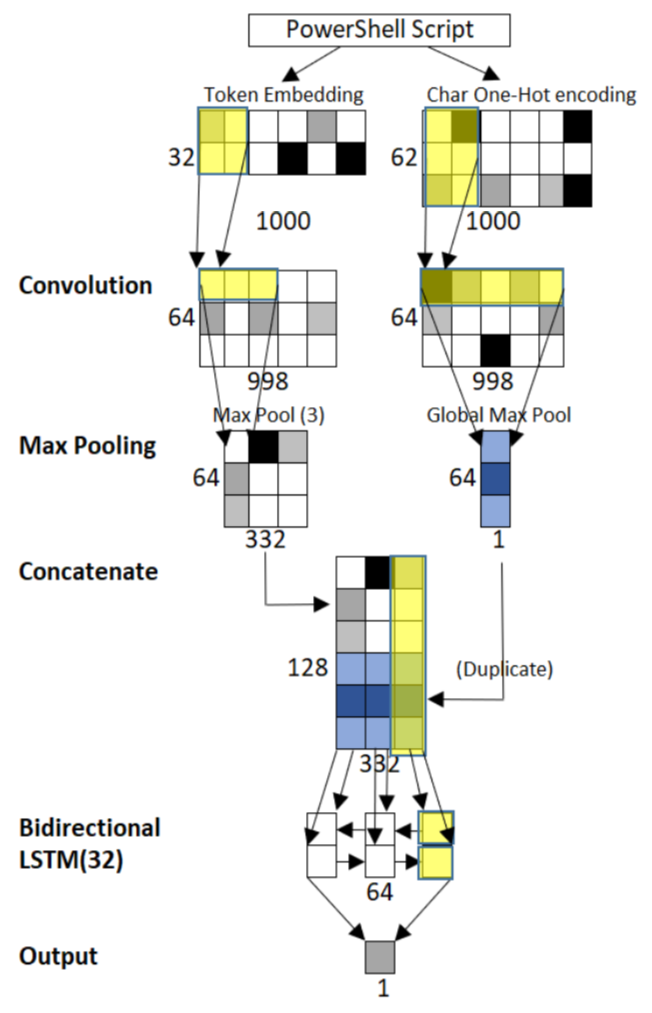
\includegraphics[scale=0.20]{inlineEnsemble}
		\caption{charCNN + CNN-LSTM model as used in \cite{amsi2019}}
	\end{figure}
\end{frame}

\begin{frame}{Lego block 3: charCNN + CNN-LSTM (2)}
	Classifier design:
	\begin{itemize}
		\item Inline ensemble of charCNN and CNN-LSTM
		\item Concatenation combines the signals from the two models
		\item Bi-directional LSTM for sequence processing
	\end{itemize}
	Other notes:
	\begin{itemize}
		\item Combination of token-based and character-based features improves performance
		\item Embedding training time = 14 hours, Classifier training time = 5 hours
		\begin{itemize}
			\item Unlabeled dataset: 368K PowerShell scripts
			\item Labeled dataset: 117K scripts (5K malicious)
			\item Azure-hosted Data-Science-VM with 56 GB of CPU memory (6 vCPUs) and 12 GB of GPU memory (single-core)
		\end{itemize}
	\end{itemize}
\end{frame}

\begin{frame}{Lego block 4: character-level 3-gram + TF-IDF + Logistic regression}
	\begin{figure}
		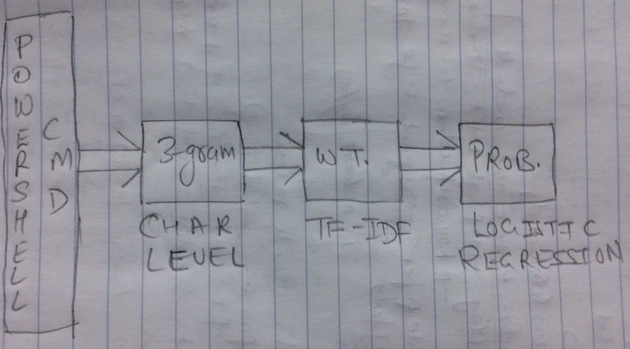
\includegraphics[scale=0.50]{3gram-tfidf-logistic}
		\caption{Traditional NLP technique as used in \cite{amsi2019}}
	\end{figure}
\end{frame}

\begin{frame}{Reported performance}
        While holding false positive rate $\le 10^{-3}$, true positive rate on held-out test set:
        \begin{itemize}
		\item charCNN: 0.799
		\item CNN-LSTM: 0.894
		\item Character-level 3-gram + TF-IDF + Logistic regression: 0.667
        \end{itemize}
\end{frame}

\begin{frame}{Lego block 5: obfuscation detector (1)}
	\begin{figure}
		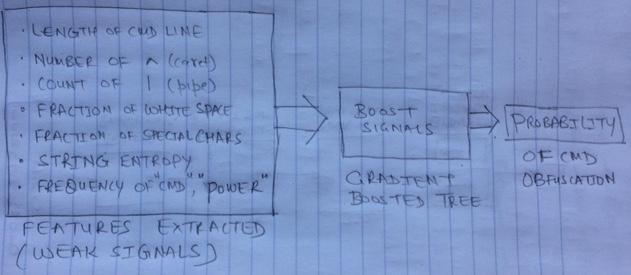
\includegraphics[scale=0.50]{gbtree}
		\caption{Obfuscation detection model as used in \cite{feye2018}}
	\end{figure}
\end{frame}

\begin{frame}{Lego block 5: obfuscation detector (2)}
	Classifier design:
	\begin{itemize}
		\item No explicit encoding or embedding
		\item Manually extracted features
		\item Traditional machine learning classification technique (gradient boosted trees)
	\end{itemize}
	Other notes:
	\begin{itemize}
		\item Classifier as described detects obfuscation (not maliciousness)
	\end{itemize}
\end{frame}

\section{Potential for new work}

\begin{frame}[fragile]{Ideas for new work}
	\begin{itemize}
		\item Transformer model \cite{transformers2019}
		\item Enhance character-level 3-gram + TF-IDF + Logistic regression (or identify alternate easily-interpretable base model with reasonable performance)
	\end{itemize}
\end{frame}

\begin{frame}[standout]
  Questions?
\end{frame}

\appendix

\begin{frame}[allowframebreaks]{References}

  \setbeamertemplate{bibliography item}{\insertbiblabel}
  \bibliography{cmd}
  \bibliographystyle{alpha}

\end{frame}

\end{document}
